%\documentclass[letterpaper,10pt]{article}
\documentclass[letterpaper,final,peerreview,10pt,onecolumn]{IEEEtranTCOM}

\usepackage{url}
\usepackage{graphicx}
\usepackage{color}
\usepackage{colortbl}
\usepackage{float}
% For reading with less pages wasted uncomment the next line
% 2012 Jan 27 commented out as per editor request
%\usepackage[margin=0.7in, paperwidth=8.5in, paperheight=11in]{geometry}
% For doublespacing uncomment the next 2 lines
\usepackage{setspace}
%\doublespacing
%\floatstyle{boxed} 
\floatstyle{ruled} 
\restylefloat{figure}
\normalsize
\hyphenation{op-tical net-works semi-conduc-tor}

\begin{document}

% Title can use linebreaks \\ within to get better formatting as desired
\title{Enhanced IP}
\date{April 17, 2012}
\author{William~Chimiak,~\IEEEmembership{Senior Member,~IEEE,}\\ Samuel~Patton,\\ and~Stephen~Janansky}
%\author{William~Chimiak, Stephen~Janansky, Samuel~Patton }

% The paper headers
%\markboth{IEEE Computer}%
%{Submitted paper}

% make the title area
\maketitle


\begin{abstract}
This paper introduces an extension to IPv4 called Enhanced IP, or EnIP for
short.  EnIP offers a solution to IPv4 address depletion. EnIP
does not replace IPv4 but builds on top of it, maximizing backward
compatibility.  EnIP is currently deployed between two nodes at the University
of Maryland and the University of Delaware, connected via Internet 2.
Each network has an IPv4 gateway with hosts behind the gateway.
Packets between the two networks are routed over IPv4 but using addresses
of the following form: 65.127.221.1.10.1.1.1.  The first four bytes
is the gateway address and the second four bytes, carried in an IP option, is
the address of a host behind the gateway.  
  
Applications such as http, samba, and ssh have been demonstrated between 
the two EnIP networks \textbf{without modification} of the software or routers 
in the path.
\end{abstract}


\section{Introduction}

%\IEEEPARstart
Enhanced IP (EnIP), provides a model for increasing the
life of IPv4 by integrating EnIP into the current
IPv4 infrastructure.  One powerful feature of EnIP is that it
does not require updates to DHCP, ARP, and existing IPv4 routing
protocols.  EnIP packets transit the Internet as IPv4 packets
carrying additional address bits and state in an IP option, so
there is no need for a routing table update as is the case in IPv6.
However, EnIP's use of an IP option requires minor additional logic to
be added to fast path implementations on routers\cite{router01}.

\section{Outline}
In parallel to Enhanced IP research, a survey paper covering many aspects
of IPv4, IPv6, and Carrier Grade NAT was created.  The survey paper is used
to justify research on Enhanced IP.  The title of the survey paper is:
Survey of Deployed Methods for Increasing Internet Address Space.  For those not familiar with the transition
to IPv6 and the evolution of IPv4, it is recommended that the survey paper
be read prior to this paper.

Section III of this paper describes the design decision to use IP options in EnIP.
Section IV introduces the mechanics of EnIP, followed by section V which
discusses the integration plan for EnIP.  
The final section includes closing remarks with emphasis on some areas
for further research.

%\include makes a pagebreak
%\nopagebreak
\section {A Survey of Layer 3 Protocol Transitions}
%\paragraph{}
The following section discusses transitions within three major
protocols of the Internet Protocol Suite. The transitions discussed
are NCP to TCP/IP, IPv4 Classless Numbering, Network Address
Port Translation (NAPT usually called NAT), Carrier Grade NAT,
and the current transition involving IPv6.

\subsection{NCP to TCP/IP}
NCP was a protocol that preceded TCP/IP as a transport protocol
on the ARPANET.  In November 1981, Jon Postel wrote RFC 801, which
described the NCP to TCP/IP transition plan.  The goal was to eradicate
NCP's usage on the ARPANET and replace it with TCP/IP.  The plan was
to begin the transition on Jan 1, 1982 and end the transition with
all hosts running TCP/IP on Jan 1, 1983.  During the transition
there would be hosts running TCP/IP, hosts running NCP only, and
hosts running both NCP and TCP/IP.  Hosts running NCP and TCP/IP
were called ``dual protocol hosts'', which is similar to language
used in the IPv6 transition standards for hosts that are dual stack,
running both IPv4 and IPv6.  The transition from NCP to TCP/IP is sometimes referred to as a flag
day because there was a date when the transition was to be finished.
At the end of the transition, the IMPs would be updated with a
simple patch to stop passing NCP.  Not all sites were preparing to
convert to TCP/IP, ``so Cerf, Postel, and the TCP/IP team turned off
the NCP network channel numbers on the ARPANET IMP's for a full day
in mid-1982''\cite{Imp01}.  They also turned off NCP for two days
later that fall.  The full switchover to TCP/IP occurred on Jan 1,
1983 without too many problems although a few sites were down for
as long as three months while they upgraded their systems.

\subsection{IPv4}
Originally, the 4 byte IP address was divided into the
\textit{network number field} (the most significant 8 bits) and the
\textit{rest field}(the lower 24 bits).  This original addressing
system only allowed for 254 different networks on the Internet which
lead to the introduction of classful network addressing in 1981
as part of the Internet Protocol (IP), RFC 791.  Classful network
addressing created three types of networks: \textit{class A},
\textit{class B}, and \textit{class C}.  Two other networks were
defined later (\textit{class D and E}).  Around 1993, RFC 1517
documented two problems caused by classful addressing.  Namely,
class C networks allowed for a network to have up to 254 hosts
while class B networks could have up to 65534 hosts.  For many
organizations, 254 addresses was not enough and 65534 was too many.
Under the classful system, organizations received a class B and
many of the addresses remained unused.  A second problem caused by
classful addressing was a large increase in the routing table size
caused by advertising many geographically dispersed class C networks.
There was no opportunity for route aggregation.  It was determined
that a change was necessary, otherwise there would be an exhaustion
of IP network numbers.  The next major evolution was to add variable
length subnet masks (VLSM).  VLSM allows networks to be divided
into smaller sizes than was possible under the classful system.  
Classless routing also introduced routing protocols that could work on arbitrary
bit boundaries.  These included RIP-2, EIGRP, IS-IS, and OSPF.

Another major change in IPv4's usage came with the introduction of 
NAT. While there are many uses of NAT, this
paper specifically refers to NAPT, which is also referred to as PAT
or IP masquerading.  RFC 2663 clarifies many terms in this 
mechanism. NAPT is the most widely used form of NAT and
the form of NAT discussed throughout this paper.  NAT allows one
or more hosts to reuse one or more public IP addresses by rewriting
packets that traverse the NAT to appear as though they originate from
the NAT's external interface.  The NAT keeps a table of port and
IP mappings so returned packets can be sent back to the internal
host that originated the connection.  There are some limits to
NAT devices.  A well understood limitation is that since end-to-end
connectivity is broken, protocols which embed their addresses in a
packet's payload are broken without additional fixup modules in the
NAT device.  Protocols such as FTP and SIP are known to have problems
traversing NATs without additional effort.   A second
problem with NATs involves the limits of the multiplexing mechanism.
There are 65535 TCP ports, thus, a quick analysis might suggest that
as many as 65535 concurrent TCP connections per public NAT IP address
is possible.  However, Miyakawa mentions an upper limit of 32000
concurrent TCP connections per IP\cite{Apnic03}.  We found a Linux
IP masquerading reference which mentions a default limit of 4096
connections and an upper limit of 32000 connections if the variables
\textbf{PORT\_MASQ\_BEGIN} and \textbf{PORT\_MASQ\_END} are adjusted
in \textit{/usr/src/linux/net/ipv4/ip\_masq.h}.  However,
this reference was only relevant to 2.4 linux kernels and at the time
of this writing 2.6 and 3.0 kernels represent modern Linux kernels.
A quick look at a more recent kernel (2.6.38) indicates that the
previously mentioned file is no longer present.  It is not clear why
Miyakawa and the 2.4 linux kernel suggest an upper limit of 32000
connections.  Further investigation into modern NAT multiplexing
mechanisms might be warranted.  One of the more interesting aspects
of Miyakawa's work was his profiling of popular applications
for the number of concurrent TCP connections required\cite{Apnic03}.
For example, he noted that iTunes required 270 connections to be
open at one point in time.  Miyakawa's results are very interesting
at a time when some Internet providers are implementing a second
layer of NAT to increase the lifespan of their IPv4 address pools.
This second layer of NAT is referred to as Carrier Grade NAT or
Large Scale NAT.  While Miyakawa's results are very interesting,
it would be beneficial to recreate his experiments for verification.


Three approaches to implementing Carrier Grade NAT were
encountered during research: Nat444, Dual-Stack Lite, and
NAT64.  In all of these approaches,
the Carrier Grade NAT is configured with a number of public IP
addresses for use in NAT.  In the NAT 444 scenario, customer
equipment is allocated an RFC 1918 address on the WAN interface
instead of a public IPv4 address.  The traffic is NATed once at the
customer's location and a second time at the Carrier Grade NAT, where
a public IP address is assigned.  With Dual-Stack Lite the customer
is provided modified customer premises equipment.  The customer's
LAN is IPv4.  When packets reach the CPE default gateway, instead of
being NATed, the packets are encapsulated in IPv6 packets and carried
to the provider's Carrier Grade NAT device.   At the Carrier NAT the
original IPv4 packets are removed from the IPv6 packet and NATed
with a public IP address.  A state table is maintained in order
to send return packets back to the appropriate CPE IPv6 address.
NAT64 requires the customer network to be completely IPv6 and all
connections to be originated by a DNS request.  When the customer
wishes to connect to an IPv4 address, such as a web site, the
customer machine issues a AAAA DNS request, which is received by
a DNS64 server.  The DNS64 server takes the request and since it
is also connected to the IPv4 network performs an A record lookup.
Once the A record lookup is returned, the DNS64 server returns a AAAA
response embedding the A record's answer in the least signficant
32-bits of the 128-bit AAAA record response.  The most significant
96-bits assures the packet will route to the NAT64 gateway.  When the
client sends the IPv6 packet it is received by the NAT64 gateway,
a router connected to both the IPv4 and IPv6 networks.  The NAT64
gateway translates the packet into an IPv4 packet and maintains a
state table for any packets that return.  In this way, an IPv6-only
host can reach IPv4 servers.  There are other translation protocols
in use not covered here but mentioned in an attempt to be complete.
They are: IVI, gogo6, Nat66, 4rd, and Nat46.

Miyakawa's work is useful for taking a population of users and
estimating the number of public IP addresses required on a Carrier
Grade NAT to accomodate $N$ customers.  Miyakawa also provides
some insight into the economics of Carrier Grade NAT.  He notes
it will be necessary to charge users less and CGN service will be
more expensive to operate because of logging.  There are
logging complexities with DS-Lite, 
but Doyle also notes logging packets in
Nat444 scenarios may not be more expensive.  Liu et. al. confirm
the technical and economic difficulties of logging Dual-Stack
Lite and NAT64 networks\cite{Nat03}.  Another interesting aspect
of Carrier Grade NAT is that in some scenarios it may make the
transition to IPv6 more difficult.  From current research, it is
not clear how Dual-Stack Lite and NAT64 affect a future transition
to IPv6, Nat 444 breaks a number of the IPv6 transition protocols.
NAT 444 appears to be the simplest of the CGN options to employ.
It is not clear how widely deployed any of the CGN technologies
have become and whether the complexity and cost of logging will
force the market to seek alternative solutions.

\subsection{IPv6}
A group known as IPng (IP Next Generation) was chartered to
create a competition focused on finding a suitable replacement
for IPv4 in RFC 1550.  RFC 1454 discusses three main protocols in the
competition: SIP, PIP, and TUBA.  The group selected
a modified version of SIP called Simple Internet Protocol Plus
(SIPP) explained in RFC 1710.  SIPP extended the address size from 32 to
64 bits.  RFCs 1883 and 2460 reflects the decision
to increase SIPP's address size from
64 to 128 bits.  In addition to a vastly
increased address size in IPv6, RFC 2460 describes how
the IPv6 header has been optimized
for routing.  This was done by removing the checksum
from the IPv6 header.  In IPv4, every time a packet traverses a
router, the IP ttl is decremented and the checksum invalidated.
The checksum must be recomputed before the packet can be forwarded.
With IPv6, recomputing the checksum is not necessary.  However,
IPv4 proponents could argue from RFC 1141 that
there are optimized implementations of
the IP time-to-live (ttl) decrement and checksum update algorithm.
Further analysis is required but perhaps this optimization is lost
from the increased computational complexity of performing the most
specific match to find an entry in the IPv6 routing table?

IPv6 provides a much larger address space, which at the
present time seems necessary given the depletion of IANA's
usable IPv4 address pool.  However, the transition to IPv6 is
non-trivial.  Few disagree with the goal of providing a larger
address pool but many have been critical of the IPv6 transition
process\cite{Cpe01,ipv6mess}.  There are
presently 292 RFC documents with the word IPv6 in the title.  It is
difficult to determine which of these documents represents the
leading thoughts on IPv6 and which documents can be safely ignored.
The task of becoming familiar with the protocols that make up IPv6
is large.   What follows is a discussion of the IPv6 transition using
five catergories: transitioning the core, transitioning the edge,
deployment to end hosts, transitioning applications, and security.

The core of the Internet operates through a number of voluntary
agreements where Internet service providers agree to allow packets
to flow between their networks.  A large tier
1 provider such as Level 3 has over 3000 BGP peering sessions,
which represent some number of business agreements less than or
equal to 3000.  Each business agreement involves the
setup of a BGP connection between providers for exchange of routes.
Typically, this is done with phone and/or email contact to setup
the BGP session.  For the IPv6 transition, providers like Level3
must obtain an IPv6 allocation, perform address planning to assign
IPv6 addresses to all relevant interfaces of their routers, and
contact their peers to setup a BGP session for the exchange of IPv6
routes.  Their peers also must obtain an IPv6 address allocation,
perform address planning, and assign addresses to the relevant
network interfaces before the exchange of IPv6 routes can occur
\cite{Peering02}.  An attempt was
made to determine the number of IPv6 autonomous systems advertising
routes into the IPv6 routing table.  In order to do this, three
bgp monitoring sources were queried.
Each of the three sources provide different numbers for the number of
IPv4 and IPv6 autonomous systems.  The numbers found are as follows:

\begin{table}[htp]
\begin{center}
\begin{tabular}{| l | c | c | c |}
\hline
 & \textbf{Date} & \textbf{IPv4} & \textbf{IPv6}  \\
\hline
 \textbf{potaroo} & October 2011 & 25296 & 741  \\
\hline
 \textbf{bgpmon} & August 2011  & 32768 & 2628 \\
\hline
\textbf{he.net} & August 2011 & 38604 & 4471 \\
\hline
\end{tabular}
\caption{Disagreement on the number of AS's in the routing tables}
\label{tab:template}
\end{center}
\end{table}

The bgpmon numbers indicate 7\% of the IPv4 autonomous systems have
enabled IPv6 and are advertising their routes into the IPv6 routing
table.  However, the potaroo numbers indicate that .029\% of the IPv4
autonomous systems are advertising IPv6 routing information while
the Hurricane Electric numbers indicate 11.6\%.  No conclusions were
drawn based on these numbers.  A discussion on IPv6 opportunities by
Vinton Cerf to the Google IPv6 Implementer's conference references 
IPv6 peering as one of the areas where more
work needs to occur.  He suggests providers should
enable IPv6 on the interfaces where there is already IPv4 peering
and that no additional peering agreements are necessary.  Cerf has
also discussed problems with home routers supporting IPv6, indicating
there is lack of a business incentive.  Standards that describe IPv6
in CPE devices began to appear in 2010\cite{Cpe02,Broadband01}.
For example, the Broadband Forum published TR-124 in May, 2010.
This document describes functional requirements for Broadband
residential gateways.  As part of this document, 22 IETF RFCs are
listed as required for meeting IPv6 requirements\cite{Broadband01}.
The IETF also describes basic requirements for customer edge routers
in RFC 6204, which was published in August, 2011.
While a few CPE devices have supported IPv6 for a while \cite{Cpe01},
there have also been a number of problems with lack of support
or broken IPv6 support in CPE implementations\cite{Cpe01,Cpe02}.
For example, some vendors of CPE devices include 6to4 support,
which is a transition technology for reaching the IPv6 Internet by
tunneling over IPv4 to an anycasted server.  Some vendors shipped
their equipment with 6to4 enabled by default which led to a number
of problems outlined in RFC 6343.  There are thirty three 6to4
gateways on the bgpmon web site.  Little information
is available in terms of the maximum load these nodes are capable
of handling.  It is not clear whether RFC 6204 or the Broadband
Forum standards represent the correct IPv6 IETF implementation.
It is not clear, why new standards are
required for CPE devices since they are routers.

With respect to deploying IPv6 to end hosts, many modern
operating systems support device configuration via neighbor
discovery as detailed in RFC 2461 and DHCPv6 described in RFC
3315.  However, one problem is that not all operating systems 
support both neighbor discovery and DHCPv6.  
As a result, it might be
necessary to choose an address assignment strategy where some
legacy operating systems can not receive IPv6 addresses from the
automatic mechanisms.

IPv6 requires some legacy software to be updated.  For example,
if a program uses \textit{gethostbyname} for dns lookups, it
will be necessary to migrate the application to use the newer
\textit{getaddrinfo} function.  \textit{getaddrinfo} returns a
\textit{struct sockaddr\_in6} if the dns resolver gets an answer
to a AAAA lookup.  It is the job of the application to pass the
\textit{struct sockaddr\_in6} to functions like connect.  This change
is simple to make.  However, there are many applications with network
functionality that need to be upgraded to handle the IPv6 case.
It seems similar to the Y2K problem.  In Y2K there were many lines
of code to be changed.  Many of these changes were not difficult
to make.  However, when considering the universe of programs to
update, the problem seems larger.  Fortunately, the model outlined in
the IPv6 transition RFCs does not suggest the IPv4 network will go
away as explained in RFC 4213.  Instead, emphasis is placed on the importance
of the IPv4 network during the change.  This strategy is called
\textit{dual stack}, since hosts and routers will run IPv4 and IPv6
stacks at the same time.  The IPv6 transition strategy also allows
for the use of transition protocols.  The IPv6 core network will
not be fully functional in the early days.  This implies that
native IPv6 connections, or direct connections into the IPv6
Internet, will not be available to everyone.  The alternative
to a native IPv6 connection is to use a transition protocol.
Transition protocols tunnel over IPv4 to reach the IPv6 network.
Some of these protocols are:

 \begin{table}[htp]
\begin{center}
 \begin{tabular}{|l|p{4in}|}
   \hline
   \textbf{RFC \#} & \textbf{Title} \\
   \hline
   4213 & Basic Transition Mechanisms for IPv6 Hosts and Routers (6in4)\\
   \hline
   3056 & Connection of IPv6 Domains via IPv4 Clouds (6to4)\\
   \hline
   4214 & Intra-Site Automatic Tunnel Addressing Protocol (ISATAP)\\
   \hline   
   4380 & Teredo: Tunneling IPv6 over UDP through Network Address Translations (Teredo) \\
   \hline
   5569 & IPv6 Rapid Deployment on IPv4 Infrastructures (6rd)\\
   \hline
  \end{tabular}
 \caption{IPv6 Transition Protocols}
\end{center}
 \end{table}

There are problems with using 6to4, 6rd, 6in4, and ISATAP from behind
NATs.  Teredo was desgined to handle this scenario.  Unfortunately,
Hoagland's study of Teredo notes it can cause unintended security
problems since it tunnels through NATs and firewalls and places
a computer directly onto the IPv6 Internet.  This is of concern
since Teredo is on by default on Windows Vista.
The availability of Teredo tunneling may
create a disincentive for ISPs to deploy Native IPv6 and for home
users to upgrade their NAT and other perimeter devices to support
the possibility of native IPv6 connectivity.

With respect to IPv6 costs, RTI prepared a report at the behest of
the U.S. National Institute for Standards and Technology suggesting
the move to IPv6 will cost U.S. entities \$25 billion over 28
years during the period 1997 to 2025\cite{RTI01}.  In addition
to estimating costs, the study also looks at potential benefits
of switching to IPv6.  One example is an estimated cost savings
from reducing NATs and the move to end to end IP reachability,
thus enabling VOIP to gain more popularity.  They estimate that
widespread VOIP usage could result in a savings of \$7.8 billion
annually.  This study has caused controversy among IPv6 proponents
who believe the roll out cost estimates are too high.
There is also belief that not enough emphasis was placed on the
costs of not switching to IPv6.  Very little information is publicly
available on the costs of upgrading software and hardware to be
compatible with IPv6.  While the costs of licensing for operating
systems based on Windows is widely available, the costs associated
with upgrading network hardware such as switches, firewalls, and
routers is not widely available in open literature.

Running a dual-stack network can increase exposure for security
vulnerability.  Neville-Neil of the Freebsd team documented a problem
in 2007 where IPv6 was partially enabled by default on Freebsd.
By default systems came up with link local addresses.  Since many
users were not aware of this behavior, their firewall rules lacked
configuration to protect the IPv6 link local address\cite{Freebsd01}.
Neville-Neil outlined how an attacker might take advantage of this.
The solution the Freebsd developers chose was to disable IPv6
in the default configuration.  Neville-Neil also mentions the
RH0 security problem.  IPv6 includes extension headers for adding
functionality to the IPv6 header much like IPv4's IP options.  One
type of routing header is the Type 0 header.  With this mechanism,
it is possible to specify the path a packet takes by specifying
IPv6 addresses as part of the routing header.  This mechanism is
similar to IPv4's loose source routing, which was itself the source
of security issues\cite{RH01}.  The IETF later deprecated support
for RH0 in RFC 5095.  There have been security issues described for
the 6to4 transition protocol.  These issues include risks for denial
of service and increased risk of spoofing IPv6 packets described
in RFC 3964.

With respect to the LAN, problems relating to the Neighbor discovery
protocols are well documented in RFCs 4861 and 4862.  For example,
RFC 6104 shows one potential problem involves rogue router 
advertisements, whether it be from misconfiguration or from a malicious person.
The attacks on neighbor discovery are similar to the attacks on ARP.
Detailed threat models for neighbor discovery are included in RFC 3756.

IPSec is included as part of IPv6 explained in RFC 2401.  There is work
on Secure Neighbor Discovery (SEND) in RFC 3971 
to address security problems outlined in RFC 3756: \textit{IPv6
Neighbor Discovery(ND) Trust Models and Threats}.
  


\section{On the Use of IP Options}
The choice to use IP options in EnIP was challenging.  During
the early stages of experimentation, IP options seemed an obvious 
choice for creating extensions to IP. However,
there were problems.  Hidell et. al. discuss the introduction
of \textbf{fast path and slow path} to routers.\cite{router02}.
With fast path, the line cards use a copy of the routing table to
make local forwarding decisions to other line cards based on table
lookups.  The fast path does not usually include the ability to
process packets containing IP options\cite{router01}.  As a result,
\textit{packets containing IP options are forwarded to the slow path}
CPU for processing and forwarding to the correct line card.

A few packets traversing the slow path should not cause saturation
of a router's CPU.  However, if EnIP were to become popular, a 
few test packets could become billions overnight and slow path CPU 
saturation could become a significant issue.  
The IP option used for EnIP has a fixed length of
12 bytes and the first byte is always 0x9a.  Presently, forwarding 
routers detect if IP options are present and send packets to the slow
path.  For EnIP packets, it would be necessary for the fast path to detect if IP
options are present, then determine if the first byte is 0x9a.  If so,
the packet is an EnIP packet and could then be simply forwarded based on 
the destination IP address using the line card's routing table.
According to Hidell et. al. routers have already moved
towards an architecture where there is flexibility in the fast path,
so this should not be difficult. 

It is known that ping packets with IP options are likely to traverse a router's slow
path. Rossi and Welzl conducted ping measurements to hosts
across the Internet and their results suggested a 10\% RTT increase
in a 2002 study, a 7\% RTT increase in a 2003 study\cite{ipopts02}
and a 26\% RTT increase in a 2004 study\cite{ipopts03}.
Fonseca et. al. studied the survivability of packets
containing IP options in an Origin AS, Transit AS, or Destination
AS\cite{ipopts01}.  Results showed packets with IP options that were
dropped, depended on the option used.
Between 85\% and 92\% of the drops occurred at an edge autonomous
system.  They showed that support for IP options in the wide area
could be restored, discovering the \textbf{core of the network
drops very few packets with options} with the majority of 
drops occurring in edge AS networks.

EnIP and IPv6 both require upgrades to the fast path implementations
of routers.  A major advantage of the EnIP approach is the
simplicity of the upgrade in comparison to the IPv6 core network
upgrade.  EnIP's fast path upgrade has the following advantages:
\begin{enumerate}
 \item No equipment reconfiguration is required (e.g. IPv6 address
 assignment, BGP configuration) 
 \item Providers can \textbf{independently} upgrade their fast paths.
 \item No updates to the IPv4 routing table are required
\end{enumerate}
    
%\documentclass[letter paper,10pt]{article}
%\usepackage{float}
%\begin{document}
\marginparwidth = 1in
\marginparpush = 0pt
\voffset = 0pt
\paperheight = 11in

\section{Introduction to Enhanced IP}
The Enhanced IP (EnIP) design increases IP address space.
EnIP allows up to approximately 2\textasciicircum 56 possible addresses 
in contrast to IPv6's offer of approximately 2\textasciicircum 128 addresses. 
The word approximately is used since both protocols include a few address 
ranges not available for use.  EnIP also offers a very practical path towards 
wide scale adoption.  It is this upgrade path and similarity to the existing IPv4
model that many may find valuable.

EnIP uses IP option 26 to create a twelve byte extension to the IP header.  This extension contains four bytes of overhead, 
and two four byte fields used as additional storage for the EnIP source and destination addresses.  
EnIP addresses are written as two IPv4 addresses concatenated together.

\subsection{EnIP Addressing Example}
An EnIP host addresses another EnIP host as follows:

\begin{center} 
65.127.221.2.10.1.1.2
\end{center}

\begin{enumerate}

\item In this example, 65.127.221.2 is a public IPv4 address allocated 
by one of the Internet registries.  Under EnIP, this address is called the site address.

\item 10.1.1.2 is a private IPv4 address assigned to a host behind a 
NAT.  In this case, the NAT and the host behind it have been upgraded to include
software to handle the EnIP extension to IPv4.

\item On the public IPv4 network, 65.127.221.2 is used for routing purposes.  In other words,
while the packet traverses the public network, its IPv4 destination is 65.127.221.2.  
Once the packet reaches 65.127.221.2, which is a NAT upgraded with EnIP software, the IPv4 
destination address is changed to 10.1.1.2, which is a value stored in the additional 12 bytes 
of space afforded by IP option 26.  The byte layout used for IP option 26 is defined in Figure 1.
\end{enumerate}

\subsection{IP Header with EnIP Option Header}
This is the IPv4 header along with additional space used 
by IP option 26\cite{rfc791}.
%\begin{center}
%\begin{figure}[H]
%\begin{verbatim}
%   0                   1                   2                   3
%   0 1 2 3 4 5 6 7 8 9 0 1 2 3 4 5 6 7 8 9 0 1 2 3 4 5 6 7 8 9 0 1
%  +-+-+-+-+-+-+-+-+-+-+-+-+-+-+-+-+-+-+-+-+-+-+-+-+-+-+-+-+-+-+-+-+
%1 |Version|  IHL  |Type of Service|          Total Length         |
%  +-+-+-+-+-+-+-+-+-+-+-+-+-+-+-+-+-+-+-+-+-+-+-+-+-+-+-+-+-+-+-+-+
%2 |         Identification        |Flags|      Fragment Offset    |
%  +-+-+-+-+-+-+-+-+-+-+-+-+-+-+-+-+-+-+-+-+-+-+-+-+-+-+-+-+-+-+-+-+
%3 |  Time to Live |    Protocol   |         Header Checksum       |
%  +-+-+-+-+-+-+-+-+-+-+-+-+-+-+-+-+-+-+-+-+-+-+-+-+-+-+-+-+-+-+-+-+
%4 |                Source Host Number                             |
%  +-+-+-+-+-+-+-+-+-+-+-+-+-+-+-+-+-+-+-+-+-+-+-+-+-+-+-+-+-+-+-+-+
%5 |              Destination Host Number                          |
%  +-+-+-+-+-+-+-+-+-+-+-+-+-+-+-+-+-+-+-+-+-+-+-+-+-+-+-+-+-+-+-+-+
%6 |             |              |E|E|                              |
%  |  Option ID  |     Option   |S|D|       Reserved               |
%  |      0X9a   |     Length   |P|P|                              |
%  +-+-+-+-+-+-+-+-+-+-+-+-+-+-+-+-+-+-+-+-+-+-+-+-+-+-+-+-+-+-+-+-+
%7 |                      Enhanced IP Source Address               |
%  +-+-+-+-+-+-+-+-+-+-+-+-+-+-+-+-+-+-+-+-+-+-+-+-+-+-+-+-+-+-+-+-+
%8 |                   Enhanced IP Destination Address             |
%  +-+-+-+-+-+-+-+-+-+-+-+-+-+-+-+-+-+-+-+-+-+-+-+-+-+-+-+-+-+-+-+-+
%\end{verbatim}
%\caption{The EnIP Packet}
%\label{Figure 2}
%\end{figure} 
%\end{center}


\begin{figure}[H]
\begin{center}
\caption{Header}
\label{Figure 1}
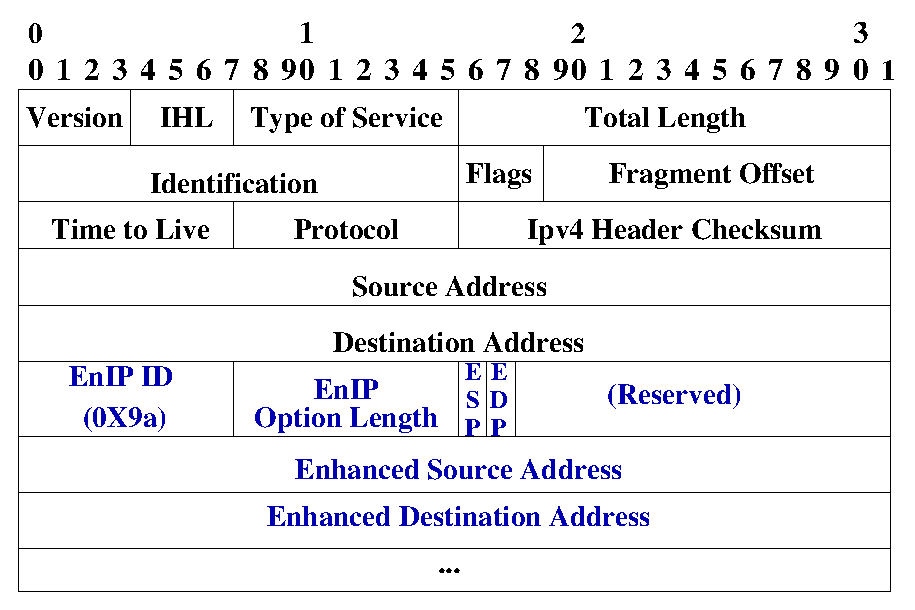
\includegraphics[scale=.5]{images/EnIPHdr.eps}
\end{center}
\end{figure} 


The EnIP ID field contains the value 0X9a.   This field can be broken down further
by converting the hexadecimal value 0x9a to binary:

\begin{center}
\textbf{1 00 11010}
\end{center}

\begin{enumerate}
 \item The first bit is a 1.  This represents the copy bit.
 \item The next two digits are 00.  This represents the \textbf{control} Option Class.
 \item The next five digits are 11010, or 26 in base 10.  This represents the new IP option value.
\end{enumerate}


If an EnIP packet traverses a router and must be fragmented because 
of a link with a smaller MTU, the copy bit ensures that fragments
include the 12 byte IP option header in each of the fragmented
packets.

In EnIP, the second byte after 0x9a is the Option Length.  This value
is always 12.  ESP and EDP are one bit fields used to indicate
whether EnIP Source Address and EnIP Destination Address are in use.
The Reserved field is unused and always set to zero.

%\begin{center}
%\begin{figure}[H]
%\begin{verbatim}
%      copy bit      Option Class          Option Value
%   +-------------+------------------+-----------------------+
%   |     1       |        00        |         01010         |
%   +-------------+------------------+-----------------------+
%   |copy bit set | Class is Control | Option is a new value |
%   +-------------+------------------+-----------------------+
%\end{verbatim}
%\caption{The EnIP Option Field}
%\label{Figure 2}
%\end{figure}
%\end{center}


The following scenarios describe the operation of EnIP, but first describe several IPv4 scenarios 
that exist today as part of a build up to help the Internet community understand the 
changes required to implement EnIP. 

Reference Figure 2 in the scenarios described below:

\begin{figure}[H]
%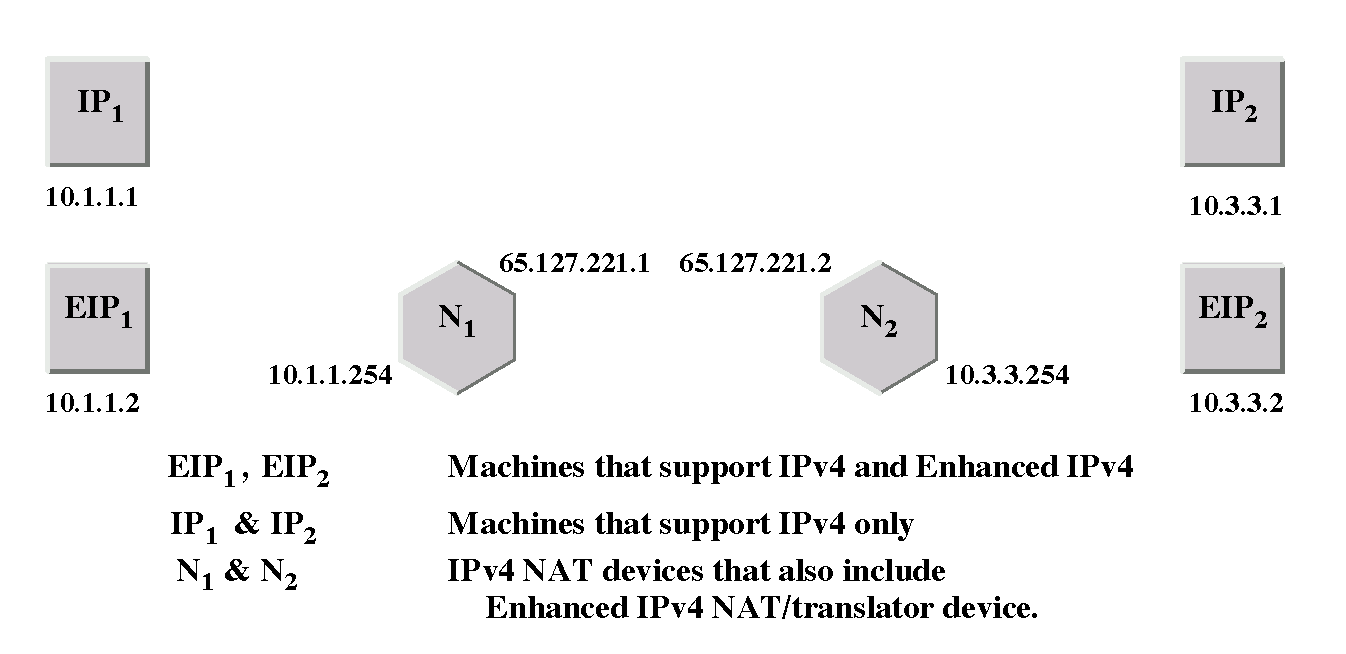
\includegraphics[scale=.7]{images/EnIPnodes.eps}
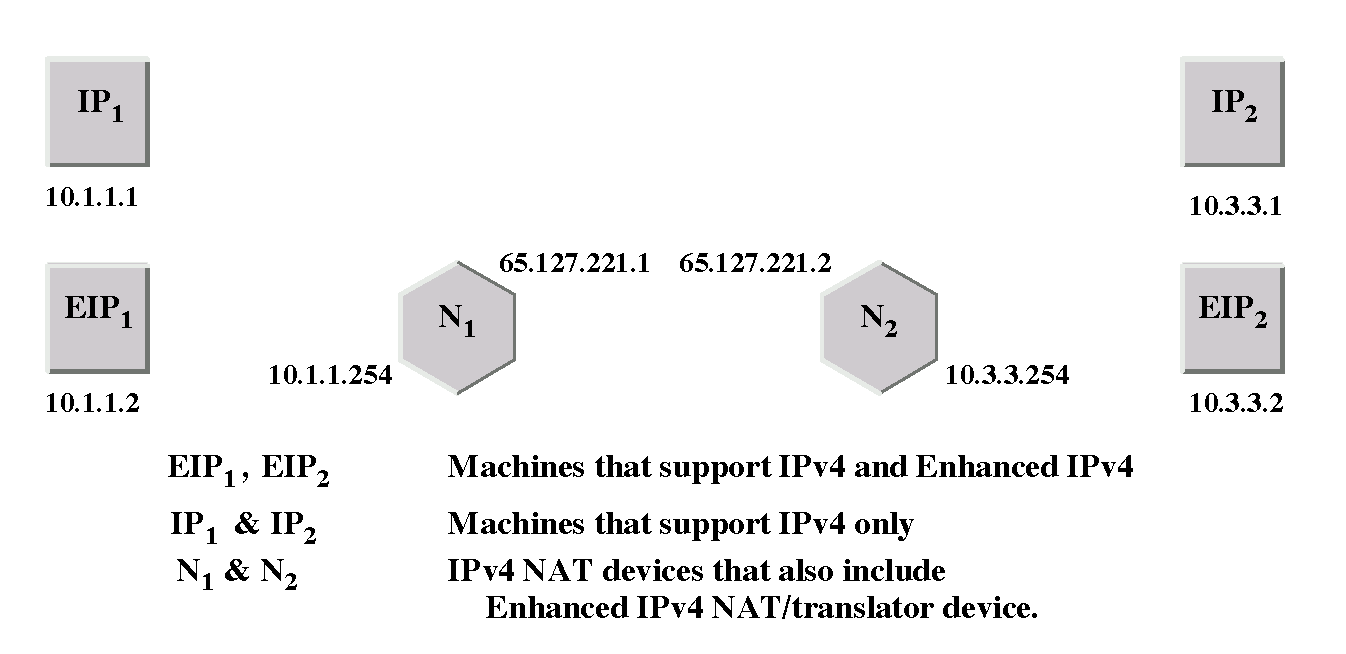
\includegraphics[height=3.0in]{images/EnIPnodes.eps}
\caption{IPv4 and Enhanced IPv4 co-existence}
% \label{fg:Xname2}
\label{Figure 2}
\end{figure}


\subsection{NAT Explanation using Figure 2}
\begin{enumerate}
 \item When IP1 (10.1.1.1), which is a host with an IPv4 stack, wants to reach 65.127.221.2 it 
  uses NAT to masquerade as the public IP address 65.127.221.1. 
  (Port-restricted cone NAT as on Linux iptables).

 \item Suppose IP1 (10.1.1.1) wants to reach tcp port 80 on IP2 (10.3.3.1), 
the packets originating from 10.1.1.1 are NAT'd by N1 to use a source IP 
address of 65.127.221.1. When these packets arrive at N2 (65.127.221.2), it is necessary 
to have a NAT port forwarding rule setup on N2 to map tcp port 80 on 65.127.221.2 
to forward packets to the internal host IP2 (10.3.3.1). This example nicely 
illustrates the power of NAT but also highlights the weaknesses of NAT to 
enable end to end host connectivity.

 \item EIP1 is a host with an IPv4 software 
stack as well as Enhanced IP extensions to IPv4. EIP stands for "Enhanced IPv4". 
Suppose EIP1 (10.1.1.2) wants to reach N2 (65.127.221.2). In this case, the 
destination IP address EIP1 will talk to is an IPv4 address (65.127.221.2). 
Because of this, the NAT device (N1) uses IPv4 NAT to translate the 
source of the packets to come from 65.127.221.1. In this case, EIP1 
behaves as though it is an IPv4 host as there is no need to use EnIP.

 \item Suppose EIP1 (10.1.1.2) wants to reach IP2 (10.3.3.1) on 
tcp port 80. In order to reach IP2, it is necessary to talk to 
N2 on address 65.127.221.2. Since this is also a function that can 
be satisfied by IPv4, when the packets from EIP1 reach N1 they 
are translated to appear as though they are coming from N1's 
external IPv4 address of 65.127.221.1. When the packets from 65.127.221.1 
reach 65.127.221.2, 65.127.221.2 must have a port forwarding entry for 
port 80 setup to send the packets to IP2 (10.3.3.1). 
It is important to note that thus far we have not demonstrated 
any usage of Enhanced IPv4 features.
\end{enumerate}

\subsection{EnIP Explanation using Figure 2}

\begin{enumerate}
\item Suppose EIP1 wants to send packets to EIP2. In this instance both hosts are running Enhanced IPv4 stacks and it is assumed that N1 and N2 support EnIP. Suppose EIP1 knows the address of EIP2 is 65.127.221.2.10.3.3.2 (more on DNS later). EIP1 knows its internal IP address of 10.1.1.2 but is not aware of the external address of N1 (65.127.221.1). Thus, initially the following is done: 
  \begin{itemize}
   \item The source IPv4 address is set to the address 10.1.1.2.
   \item The EnIP ID field is set to 0X9a.
   \item The ESP bit in the EnIP header is set to zero. 
   \item The Enhanced IP Source Address in the EnIP header is set to all ones, or 255.255.255.255, since an Enhanced IP source address is not currently present.
   \item The most significant 32 bits of the EnIP address is set by storing 65.127.221.2 in the IPv4 destination field 
   \item The least significant 32 bits of the EnIP address is set by storing 10.3.3.2 in the Enhanced IP Destination Address field.
   \item The EDP bit is set to 1.
  \end{itemize}

\item When the packet arrives via IPv4 routing to N1, N1 does the following:
  \begin{itemize}
  \item Examines the packet and determines it has the Enhanced IP options present (0x9a). 
  \item Writes the EnIP source address by reading 10.1.1.2 from the IPv4 source address field and
  placing this value in the Enhanced IP Source Address field.  This field no longer contains 255.255.255.255.
  \item  Sets the ESP bit to 1.
  \item  Places 65.127.221.1 as the IPv4 source address.
  \item  Recomputes the IP checksum of the packet since it has changed.  If the packet carries TCP or UDP, recomputes these checksums as they have also changed.
  \end{itemize}
\item Upon arrival at N2 (65.127.221.2), N2 does the following:
  \begin{itemize}
  \item Recognizes the Enhanced IP packet. (0x9a)
  \item Reads the EnIP Destination Address of 10.3.3.2 and places this value into the IP header's destination address, so that the IP destination address is now 10.3.3.2.
  \item Sets the EDP bit to 0
  \item Sets EnIP Destination Address to zero.
  \item Recomputes the IP checksum.  If the packet carries TCP or UDP, recomputes these checksums as they have changed as a result of a change to the IP destination address.
  \item N2 sends the packet to EIP2.
  \end{itemize}

  \item When EIP2 receives the packet it does the following:
  \begin{itemize}
   \item Computes the source address of the packet by concatenating the 
  IPv4 source field (65.127.221.1) with the EnIP source field (10.1.1.2) to get 65.127.221.1.10.1.1.2.
  \item The IPv4 destination address is 10.3.3.2.
  \end{itemize}

\item To construct a packet from EIP2 to EIP1, EIP2 does the following:
  \begin{itemize}
   \item  Sets the Option ID field to 0x9a.
   \item Takes the IPv4 source address field from the incoming packet, 65.127.221.1,
   and sets it as the IPv4 destination field.
   \item  Places the EnIP source address (10.1.1.2) in the EnIP Destination Address field.
   \item Set the EDP field to 1.
   \item  Sets the IPv4 source address field to 10.3.3.2.
   \item  Sets the EnIP source address to all ones (255.255.255.255), setting the ESP bit to 0.
  \end{itemize}

\item When the packet arrives at N2, the following is done by N2:
  \begin{itemize}
   \item Places 10.3.3.2 in the EnIP source address field.
   \item Set the ESP bit to 1.
   \item Place 65.127.221.2 in the IPv4 source address field.
   \item Recomputes the IP checksum and if the packet carries TCP or UDP, recompute these checksums as well.
   \item Send the packet to N1 (65.127.221.1).
  \end{itemize}

\item When the packet arrives at N1, it does the following:
  \begin{itemize}
   \item  Read 10.1.1.2 from the EnIP destination address field, and place this value in the IPv4 destination address field.
   \item  Set EDP to 0.
   \item Place a value of 0 in the EnIP destination address field.
   \item Recompute the IP checksum and if the protocol is TCP or UDP, recompute these checksums as well.
   \item Send the packet to EIP1..
  \end{itemize}

\end{enumerate}

\subsection{Upgrading Servers to Support EnIP}
An existing server deployed using an IPv4 address can be easily upgraded to support EnIP connections.
Suppose the server is a simple TCP echo server\cite{rfc862}.  The echo program creates a listening socket and then reads data from it.
Any data read from the socket is also written back to the same socket.  Without being upgraded, it should
be possible for the server to read EnIP packets from the socket.  However, it will not be possible for the server
to write EnIP packets back to the socket correctly.  The packets would only be sent to the source IPv4 address and not
back to the EnIP address which includes the source IPv4 address and the EnIP Source Address.  Once the server
has the EnIP upgrades, it will be possible for it to receive packets and send echo responses back to the full EnIP 
address that originated the packet.  Care must be taken here to ensure that the EnIP Source Address is one of the 
allowed RFC 1918 addresses.  

Suppose the echo server also logs the source IP address of each data packet received using the \textit{getpeername}
function.  The length of the address structure returned is currently either the size of a \textit{struct sockaddr\_in} (16 bytes) for IPv4
or the size of \textit{struct sockaddr\_in6} (28 bytes) for IPv6.  The ALPHA implementation of EnIP returns a new structure called
\textit{struct sockaddr\_ein}(26 bytes).  If it is desired to print out the EnIP addresses correctly, it is necessary to 
use the length 26 to detect a \textit{struct sockaddr\_ein}.  Inside this struct are two values: sin\_addr1 and sin\_addr2.  These
represent the IPv4 source address and the EnIP Source Address.  An implementation of getpeername could provide a compatibility
mode to treat EnIP addresses as IPv4 addresses.  Once the echo client software is upgraded, the getpeername implementation could
return struct sockaddr\_ein.

\subsection{DNS Operation}
RFC 2928 sets aside\cite{rfc4727} the experimental IPv6 prefix 2001:0101.  
EnIP lookups use AAAA records that begin with the experimental prefix 2001:0101.  
The prefix 2001:0101 uses 32 bits of the 128 bit AAAA record, leaving 96 bits for EnIP to 
use, of which 64 bits are used.
Supposing the EnIP address was 65.127.221.2.10.1.1.2, the EnIP AAAA record would be 2001:0101:417f:dd02:0a01:0102::0.
This use of the AAAA record is called a AA record.  It is important to note that a new AA record type was not added, rather
the AA record is a record created by retrofitting the 64 bit EnIP address into the existing AAAA record.  
With this approach, it is not necessary to upgrade DNS server software so long as it supports AAAA lookups.
It is imagined in the future, that DNS software will be upgraded to hide these details from the user.  For example,
the user might enter:

\begin{verbatim}
65.127.221.1.10.1.1.2       AA       eip1.example.com
65.127.221.2.10.3.3.2       AA       eip2.example.com
\end{verbatim}


\subsection{Optional DNS Upgrades}
Suppose EIP1 must speak to another EIP host behind N1.
Call this host EIP3. EIP3 has an address of 10.1.1.3 and like EIP1 has an 
external source address of 65.127.221.1. An important question to consider is can EIP1 talk 
to EIP3 using EnIP addressing without relaying all packets via N1?  Suppose the enterprise uses the domain name
example.com.  On the authoritative name server for example.com, the enterprise maintains a list of IP networks controlled by the
enterprise.  Suppose 65.127.221.1 is the only entry in the list.  DNS resolvers typically look up AAAA records followed by A records
if the AAAA lookup does not succeed.  If a DNS query from 65.127.221.1 arrives at the authoritative server requesting a AAAA record
for EIP3.example.com it would be possible to send back DNS answer for no such record.  When the request for the A record for EIP3.example.com
arrives at the name server, the authoritative server responds with the least significant 32 bits of the EnIP address.  When other
IP addresses query the authoritative name server asking for the AAAA record of EIP3.example.com, they will receive the EnIP address encoded as an IPv6 address.

\subsection{Security Issue: Preventing EnIP NAT or hosts from forwarding illegal packets}
EnIP-capable NAT devices swap the EnIP destination address into the IPv4 header's destination address.  Once the swap occurs the packet
is routed on to the address stored in the EnIP destination field.  This is the desired behavior when the destination address is for a network directly connected
to the NAT.  This is not the desired behavior if the NAT is forwarding on to a network that is not directly connected.  EnIP NAT devices MUST only perform
the swap and forward operation if the EnIP destination address is for an RFC 1918 address of a network directly connected to the EnIP NAT.  
To perform this swap otherwise, would mean packets sent to EnIP NATs could be used to relay packets towards
unwitting victims.  If not protected against, this could lead to these packets being used in denial of service attacks or other malicious acts.

\subsection{Security Issue: IPSEC}
EnIP breaks IPSEC in the full tunnel mode AH+ESP scenario.  NAT
already breaks this configuration of IPSEC. It is important to acknowledge this as a design limitation.  More work would be required to
modify IPSEC to work with EnIP.  

\subsection{Security Issue: Host security, sensible defaults}
EnIP hosts behind a permissive EnIP NAT device are more exposed on the Internet.  It is recommended that the default configuration
of an EnIP NAT not allow any inbound connections to EnIP hosts behind the NAT unless explicitly configured to do so.  This is the most sensible configuration
for EnIP devices designed for the home user as replacements/upgrades to existing NAT gateways.  This configuration will not be possible for the
mobile network.

%\end{document}
     %bill
\section{EnIP Integration}
Currently, mobile devices are the largest growing consumers of IP
addresses.  EnIP Integration begins by focusing on 
the steps to enable Enhanced IP for Mobile Devices.  Mobile service
providers could benefit from the ability to address any phone
with a unique IP address.  This is not possible with IPv4.
This would be possible with Enhanced IP.  It is envisioned that Enhanced
IP would enable VoIP systems to make calls based on 64-bit EnIP
addresses.

\paragraph{Phase 1: Deployment to Mobile Devices and Infrastructure}
Technologies such as LTE and WiMAX provide voice channels, previously
circuit switched, using Internet protocols (mainly Voice over IP or
VoIP).  This can stress a provider's overloaded NAT devices and usually requires
NAT traversal methods such as STUN to enable end-to-end communications.

NATs are typically limited on the number of devices they can
support based on the number of active ports used.  There are
only 65,535 ports available. So at best one IP can only sustain that
many connections for devices it serves.  A large amount of loaded
persistent connections can degrade NAT service.  Voice channels are
sensitive to these degradations.  EnIP resolves these for providers
due to it's stateless nature and ability to allow for end-to-end
communication.  EnIP on mobile devices is the proposed first stage of
integration.

EnIP's deployment to mobile devices should be straightforward
for all stakeholders.  For simplicity, consider the Android Open
Source Platform.  Given Android's Linux core, EnIP patches written
against the Linux Kernel are merged into a release of Android.
Device manufacturers provide carriers with their updated Android
device firmware release.  Service providers utilize their established
firmware update mechanism, updating their customers'
devices.  Legacy NAT traversal techniques are used with old
IPv4 devices for which an EnIP update is not available.  After a kernel
update the new devices are ready to communicate over EnIP.

The next step in phase 1 is for a service provider to upgrade their networks
to support EnIP.  To do this, providers first apply the EnIP NAT
patch to their NAT devices.  This involves a small modification
of the NAT kernel moduel (nf\_nat.ko) and the addition of another (eipnat.ko). 
We have demonstrated it is possible to perform this update without rebooting a
NAT server.  Next, providers update
their intermediate connections between provider networks to allow
for the passing of IP Option 26.  In addition to this, router fast paths will 
need to be updated so that IP Option 26 is no longer passed via the slow path.
Once completed, mobile devices can
perform device-to-device communication using EnIP.  EnIP connections
do not deplete the number of connections available on a NAT as
is the case with current VOIP architectures that utilize IPv4 and NAT.

It is possible for EnIP to be a successful protocol completely within the 
confines of mobile networks.  It is envisioned that mobile operators will use
EnIP to create end-to-end VoIP systems.

\paragraph{Phase 2: Deployment to Content Providers and Infrastructure}
A move of mobile devices to EnIP initially benefits mobile
providers by making simpler VoIP architectures possible.  The remaining traffic
transitting their NATs is data traffic to and from content providers.  In particular,
the large content providers produce most of the traffic.
The steps for content providers to support
EnIP are simple enough that this integration is realistic.

Content providers upgrade in two steps:  First, they integrate EnIP
into their networks.  IP Option 26 must be allowed to traverse
their networks and the fast paths of their routers must be upgraded to
quickly process EnIP packets.
All routers MUST process EnIP packets in the fast path.
Network equipment vendors should make these fast path upgrades available.  
Vendors not providing an upgrade place themselves at a competitive disadvantage.
Since many of these vendors have the experience of designing fast path
upgrades for IPv6, the minor changes required for EnIP integration should be simple.
Similarly, NAT implementations should begin to integrate EnIP.  It will also be 
necessary to upgrade firewall software in some cases so it can forward packets 
containing IP Option 26.  With this completed,
traffic can successfully traverse between content providers and
mobile customer networks.  Since the customers will already be
able to communicate over EnIP, and the packets can now flow between
provider and customer, it will be time to upgrade the servers which
provide the content.

The second step in Phase 2 is to perform an upgrade to the servers
and software which provide the content.  EnIP patches for the host
operating systems need to be deployed.  These patches are minimal and
comparable to the application of small security patches.  In Linux,
for example, it will require short patches of approximately 700
lines of code to the system's kernel in order to allow it to properly
process EnIP connections.  Once this is completed and
verified, applications need to be tested.  Our initial application
tests worked without modification(ssh, samba, apache, firefox).  
Once applications are validated,
content providers switch to the integrated EnIP-IPv4 setup allowing
them to serve both legacy IPv4 customers and the newer EnIP customer set.

\paragraph{Phase 3: Deployment to Last Mile and Home Users}
First, ISPs integrate EnIP into their core and edge devices, as
the content providers did.  Then they upgrade the Customer Premise
Equipment when additional address space is needed.  In cases where
the users own their CPEs, the vendors provide firmware updates and
users upgrade their devices.  For those who have ISP provided CPEs, the
ISP can patch the devices' NATs to support EnIP.  As before, the
patches are small so ISPs can upgrade their customer devices without
rebooting the devices.  At this point, mobile devices will be capable
of utilizing their home network for backhaul to Mobile Providers.

With the user's home network capable of passing EnIP, users could
start to make use of the protocol on their computer systems
as well.  Patches to the host OS could be provided through
auto-update procedures to all major Operating Systems.  At this
point, home users could opt-in to using EnIP on their home network,
if they wish.  Some mobile service providers who also offer home Internet services
may be motivated to upgrade some home users CPE devices early so that mobile device
voice calls can be offloaded to a wireline connection.
 %steve
\section{Conclusion}
This paper described several migrations and modifications to solve
problems that arose in the Internet Protocol suite.  The NCP to TCP
transition was very disruptive and possible at a time when not many
people, governments, and businesses were dependent on the network.
It is difficult to imagine deploying a new Internet protocol using a flag 
day approach.  The migration to classless addresses
was beneficial and not disruptive.  Network Address Port Translation
developed out of necessity and solved many privacy and address
problems and admittedly created some minor ones.  IPv6 seems to
be disruptive and its implementation appears difficult.  The days of
experimenting on the network anywhere at anytime are long over.  There are
too many people and livelihoods dependent on the network for critical
services.  The next transition must be simple.  This literature survey is used as the basis 
for further research on IP extensions.  Specifically, it was used to 
inform research on another protocol known as Enhanced IP.
	

\bibliographystyle{plain}
\bibliography{ourrefs,rfc}

\end{document}
